\documentclass{article}

%%%%%%%%%%%%%%%%%%%%%%%%%%%%%%%%%%%%%%%%%%%%%%%%%%%%%
%                                                   %
%              Template by Tuur Vanhoutte           %
% https://github.com/zjeffer/howest-thesis-template %
%                                                   % 
%%%%%%%%%%%%%%%%%%%%%%%%%%%%%%%%%%%%%%%%%%%%%%%%%%%%%

%%%%% Package importing %%%%%
\usepackage[english]{babel}
\usepackage[margin=2.5cm]{geometry}
\usepackage{graphicx}
\usepackage{float}
\usepackage{caption}
\usepackage{hyperref}
\usepackage{amsmath}
\usepackage{wrapfig}
\usepackage[parfill]{parskip}
\usepackage{eso-pic}
\usepackage{titlesec}
\usepackage{titletoc}
\usepackage{tcolorbox}
\usepackage{enumitem}
\usepackage{changepage}

\usepackage{bookmark}
\usepackage{csquotes}
\usepackage[style=ieee]{biblatex}
\addbibresource{sources.bib}


%%%%% Change fonts here %%%%%
\usepackage[T1]{fontenc}
\usepackage{helvet}
\renewcommand{\familydefault}{\sfdefault}

\graphicspath{{img/}}

%%%%% \theorem environment %%%%%
\usepackage{amssymb}
\newtheorem{theorem}{Definition}[section]
\newenvironment{thmenum}
 {\begin{enumerate}[label=\upshape\bfseries(\roman*)]}
 {\end{enumerate}}


%%%%% Styled code block %%%%%
\usepackage{minted}
\setminted{frame=single,framesep=3pt,linenos}
\usepackage{upquote}
\usepackage{color}

%%%%% TOC styling %%%%%
\makeatletter
\renewcommand\tableofcontents{%
  \null\hfill\textbf{\Huge\contentsname}\hfill\null\par
  \vline\noexpand\rule{\textwidth}{1pt}%
  \@mkboth{\MakeUppercase\contentsname}{\MakeUppercase\contentsname}%
  \@starttoc{toc}%
}
\makeatother

\begin{document}

%%%%% title page %%%%%
\begin{titlepage}
    \newgeometry{margin=0cm}
    \begin{center}
        %%%%% Change the cover image here %%%%%
        \includegraphics[width=18.5cm,height=18.5cm]{example-image}
    \end{center}
    \begin{adjustwidth}{1.5cm}{1.5cm}

    \vspace{0.5em}

    \MakeUppercase{\Huge\textbf{How to create a chess engine using Deep Reinforcement Learning}}

    \MakeUppercase{\Large\textit{A critical look at DeepMind's AlphaZero}}

    \vspace{1em}

    \MakeUppercase{Internal promotor: Wouter Gevaert}

    \MakeUppercase{External promotor: <name here>}

    \vspace{1em}

    \MakeUppercase{\small{Research conducted by}}

    \MakeUppercase{\Large\textbf{{Tuur Vanhoutte}}}

    \MakeUppercase{\small{for obtaining a bachelor's degree in}}

    \MakeUppercase{\Large{\textbf{{Multimedia \& Creative Technologies}}}}

    \MakeUppercase{Howest | 2021-2022}
    \end{adjustwidth}
\end{titlepage}

\newgeometry{margin=2.5cm}

\newpage
\thispagestyle{empty}
\mbox{}
\newpage

%%%%% Set pagenumbering off %%%%%
\pagenumbering{arabic}
\thispagestyle{empty}
%%%%% Preface %%%%%
\section*{Preface}
\addcontentsline{toc}{section}{Preface}

This bachelor thesis is the conclusion to the bachelor program Multimedia \& Creative Technologies at Howest college
West Flanders in Kortrijk, Belgium. The program teaches students a wide range of skills in the field of 
computer science, with a focus on creativity and Internet of Things. From the second year on, students can choose 
between four different modules:

\begin{enumerate}
    \item \textbf{AI Engineer}
    \item \textbf{Smart XR Developer}
    \item \textbf{Next Web Developer}
    \item \textbf{IoT Infrastructure Engineer}
\end{enumerate}

This bachelor thesis was made under the \textbf{AI Engineer} module.
The subject of the thesis is a critical look at the result of my research project 
in the previous semester. The goal of the project was to create a chess engine in Python with
deep reinforcement learning based on DeepMind's AlphaZero algorithm. 

I will explain the research I needed to create it, the technical details on how to program the
chess engine and I will reflect on the results of the project. To do this, I will contact 
multiple people familiar with the field of reinforcement learning to get a better understanding of the
impact of this research on society. Based on this, I will give advice to people and companies who 
wish to implement similar algorithms.

I would like to show gratitude to Wouter Gevaert for his enthusiastic support in the creation of my research project 
and this thesis. I also want to thank the other teachers at Howest Kortrijk, who shared their knowledge
and expertise in programming and AI in very interesting classes.

% TODO: thank external promotor

Furthermore, I would like to thank my parents for giving me the chance to have a good education, and 
the motivation to get the best I can out of my studies.

\vspace{3em}

\begin{center}
    \textbf{Tuur Vanhoutte}, 1$^{\text{st}}$ June 2022 % TODO: verander datum naar datum finale versie
\end{center}

\newpage
\thispagestyle{empty}
\mbox{}
\newpage

%%%%% Abstract %%%%%
\section*{Abstract}
\addcontentsline{toc}{section}{Abstract}


% TODO: abstract verder aanvullen

% Samenvatting of abstract (mag in het Engels): MAX 1 halve A4-pagina: 
% Je beantwoordt in de samenvatting kort en bondig een viertal vragen: 
% X Wat is de onderzoeksvraag?
% X Wat was jouw onderzoek? 
% - Welke elementen spelen een grote rol (zowel positief als negatief) bij de evaluatie van het onderzoek? 
% - Welke elementen zijn belangrijk bij jouw advies?
% - Het besluit wordt kort samengevat

This bachelor thesis answers the question: ``How to create a chess engine using deep reinforcement learning?''.
It explains the difference between normal chess engines and chess engines that use deep reinforcement learning, and
specifically tries to recreate the results of AlphaZero, the chess engine by DeepMind, in Python on consumer hardware. 

The technical research shows what is needed to create my implementation using Python and TensorFlow. 
It shows how to program the chess engine, how to build the neural network, and how to train and evaluate the network.
During the creation of this chess engine, it was crucial to create a huge amount of data through self-play.

The thesis contains a reflection on the results of my research project, which proposes a solution to the problem of
creating a high amount of games through self-play. It also reflects on the impact of this research on society, and the
viability of this type of artificial intelligence in the future. With this comes a section on advice for companies that wish
to implement similar algorithms.

% It concludes... (TODO)


\newpage
\thispagestyle{empty}
\mbox{}
\newpage

%%%%% Table of contents %%%%%
\addcontentsline{toc}{section}{Contents}
\tableofcontents
\newpage

%%%%% List of figures %%%%%
\section*{List of figures}
\addcontentsline{toc}{section}{List of figures}
\renewcommand{\listfigurename}{}
\listoffigures
\newpage

% TODO: Remove if no tables
% \section*{List of tables}
% \addcontentsline{toc}{section}{List of tables}
% \renewcommand{\listtablename}{}
% \listoftables

%%%%% List of abbreviations %%%%%
\section*{List of abbreviations}
\addcontentsline{toc}{section}{List of abbreviations}



%%%%% Glossary %%%%%
\newpage
\section*{Glossary}
\addcontentsline{toc}{section}{Glossary}

%%%%% Introduction %%%%%
\newpage
\setcounter{section}{0}
\section{Introduction}

% Doel: In de inleiding beschrijf je ook hoe jouw bachelorproef in elkaar steekt. Een krachtige heldere inleiding 
% zorgt ervoor dat je de lezer voor je wint en hij/zij sneller de rest van jouw document zal gaan lezen. 
% In de inleiding introduceer je de onderzoeksvraag. Je vermeldt de achtergrond of bestaande situatie. Je licht toe 
% waarom de onderzoeksvraag voor jou/jouw stagebedrijf relevant is. Ook eventuele deelvragen worden 
% nauwgezet omschreven. 
% De inleiding omschrijft ook de gebruikte onderzoeksmethode. Je legt uit waar, wanneer, met wie en hoe je het 
% onderzoek gaat doen. 
% Je kunt alvast gebruikmaken van één of meerdere standaardzinnen: 
% - De data voor dit onderzoek zijn verzameld door... 
% - Vijf stukken worden onderzocht, die allemaal... 
% - De onderzoeksgegevens in deze bachelorproef zijn afkomstig uit vier belangrijke bronnen, namelijk... 
% - Door kwalitatieve methoden te gebruiken probeer ik... uiteen te zetten/uit te lichten. 
% - De studie is uitgevoerd in de vorm van een enquête, waarbij data zijn verzameld via... 
% - De methode die in deze studie gebruikt is, is een gemengde aanpak gebaseerd op...

Chess is not only one of the most popular board games in the world, it is also a breeding ground for
complex algorithms and more recently, machine learning. Chess is theoretically a deterministic game: 
no information is hidden from either player and every position has a calculable set of possible moves.
Because the branching factor of chess is about 35-38 moves \cite{BranchingFactorChessprogramming}, 
calculating if a position is winning or losing requires an enormous amount of calculations.

Throughout the entire history of computer science, researchers have continuously tried to find better
ways to calculate if a position is winning or losing. The most famous example is the StockFish 
engine \cite{StockfishChess2022}, which uses the minimax algorithm with alpha-beta pruning to calculate the best move.

More recently, researchers at Google DeepMind have developed a new algorithm called AlphaZero \cite{AlphaZero2022}.
This thesis explores the concept of AlphaZero, how to create a chess engine based on it, and the impact of 
the algorithm on both the world of chess and the rest of society.

Research has been conducted by investigating what is needed to recreate the results of AlphaZero, 
by programming a simple implementation using Python and TensorFlow. This was done as part of a research project
between November 2021 and January 2022. The code was written with lots of trial and error, as DeepMind released 
very little information about the detailed workings of the algorithm. 

% TODO: more info


%%%%% Add Howest background %%%%%
\AddToShipoutPicture{
    \ifnum\value{page}>0
    \AtPageLowerLeft{
    \raisebox{3\baselineskip}{\makebox[0.25\paperwidth]{
        \begin{minipage}{21cm}\centering
            
\includegraphics{img/background.png}
        \end{minipage}}}
    }
  \fi
}

%%%%% Research %%%%%
\newpage
\section{Research}

%%%%%%%%%%%%% 
% 
% Answer the theoretical questions:
%
% [ ] Hoe kan ik het Monte Carlo Tree Search algoritme gebruiken om de beste zetten te selecteren?
% [ ] Welke voordelen biedt deep reinforcement learning bij schaken?
% [ ] Hoe ziet de architectuur van het neurale netwerk er uit?
% [ ] Hoe werd deep reinforcement learning reeds gebruikt bij andere spellen?
% [X] Hoe werken huidige schaakcomputers die geen neurale netwerken gebruiken?
%
%%%%%%%%%%%%%

\subsection{What is a chess engine?}

According to Wikipedia \cite{ChessEngine2022}, a chess engine is a computer program that analyzes 
chess or chess variant positions, and generates a move or list of moves that it regards as strongest.
Given any chess position, the engine will estimate the winner of that position based on the strength 
of the possible future moves up to a certain depth. The strength of a chess engine is determined by
the amount of moves, both in depth and breadth, that the engine can calculate. 


\subsection{How do traditional chess engines work?}

Contemporary chess engines, like StockFish \cite{StockfishChess2022}, use a variant of the minimax algorithm that employs alpha-beta pruning.

\subsubsection{The minimax algorithm}

The minimax algorithm \cite{Minimax2022} is a general algorithm usable in many applications, ranging from artificial intelligence to 
decision theory and game theory. The algorithm tries to minimize the maximum amount of loss. In chess, this means 
that the engine tries to minimize the possibility for the worst-case scenario: the opponent
checkmating the player. For games where the player needs to maximize a score, the algorithm is called maximin: 
maximizing the minimum gain. 

Minimax recursively creates a search tree \cite{eppesHowComputerizedChess2019}, with chess positions as nodes and chess moves as edges between the nodes. 
Each node has a value that represents the strength of the position for the current player. 
At the start of the algorithm, the tree only consists of a root node that represents the current position. 
It then explores the tree in a depth-first manner by continuously choosing random legal moves, creating nodes and edges in the process.

This means that it will traverse the tree vertically until a certain depth is reached:

\begin{figure}[H]
    \centering
    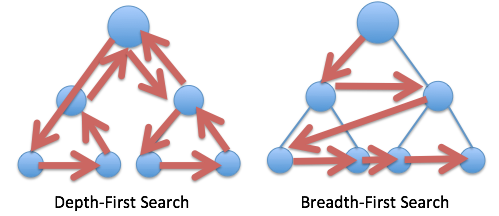
\includegraphics[width=0.5\textwidth]{img/depth-vs-breadth.png}
    \caption{Depth-First search vs Breadth-First search \cite{eppesHowComputerizedChess2019}}
\end{figure}

When that happens, that leaf node's position is evaluated and its value is returned
upwards to the parent node. The parent node looks at all of its children's values, 
and receives the maximum value when playing white, and the minimum value
when playing black. 

This repeats until the root node receives a value: the strength of the current position.

\subsubsection{The evaluation function}

The value estimation of leaf nodes is done by an evaluation function \cite{EvaluationFunction2022} written specifically
for the game. This function can differ from engine to engine, and is usually written with 
help from chess grandmasters. 



\subsubsection{Pseudocode}

The algorithm is recursive; it calls itself with different arguments, depending
on which player's turn it is. In chess, white wants to maximize the score, and 
black wants to minimize it. \cite{Minimax2022}

\begin{minted}{c}
function  minimax(node, depth, maximizingPlayer) is
    if depth = 0 or node is a terminal node then
        return the heuristic value of node
    if maximizingPlayer then
        value := - inf
        for each child of node do
            value := max(value, minimax(child, depth - 1, FALSE))
        return value
    else (* minimizing player *)
        value := + inf
        for each child of node do
            value := min(value, minimax(child, depth - 1, TRUE))
        return value
\end{minted}

Calling the function:

\begin{minted}{c}
// origin = node to start
// depth = depth limit
// maximizingPlayer = TRUE if white, FALSE if black
minimax(origin, depth, TRUE)
\end{minted}

\subsubsection{Alpha-beta pruning}

Because the necessary amount of nodes to get a good estimation of the strength of a position
is so high, the algorithm needs to be optimized. 
Alpha-beta pruning \cite{AlphaBetaPruning2022} aims to reduce the amount of nodes that need to be explored by minimax.
It does this by cutting off branches in the search tree that lead to worse outcomes.

Say you're playing the white pieces. You want to minimize your maximum loss, which means 
you want to make sure that black's score is as low as possible. 
Minimax always assumes that the opponent will play the best possible move. If one of white's possible moves
leads to a position where black gets a big advantage, it will eliminate that branch of the search tree.
As a result, the amount of nodes to explore is greatly reduced, while retaining a good estimation 
of the strength of the position.

Since 2020, StockFish has been using a sparse and shallow neural network as its evaluation function. 
This neural network is still trained using supervised learning, not (deep) reinforcement learning.

\subsection{Monte Carlo Tree Search}

The biggest problem with minimax algorithms with a depth limit is that it is very dependent
on the evaluation function you use: if the evaluation function makes an incorrect estimation, 
the algorithm will suggest bad moves. Developers of contemporary chess engines like StockFish continuously
try to improve this function. 

Using alpha-beta pruning can also bring about some problems. Say the player can sacrifice a piece
to get a huge advantage later in the game. The algorithm might cut off the branch and never explore that winning line, 
because it considers the sacrifice a losing position \cite{MinimaxMonteCarlo}. 

Monte Carlo Tree Search (MCTS) \cite{MonteCarloTree2022} is a search algorithm that can be used to mitigate these problems.
MCTS approximates the value of a position by creating a search tree using random exploration of the most promising moves.

\subsubsection{The algorithm}

To create this search tree for a certain position, MCTS will run the following algorithm hundreds of times. 
Each of these runs is called an MCTS \textbf{simulation}. One simulation consists of four steps:

\begin{enumerate}
    \item \textbf{Selection}:
    \begin{itemize}
        \item Starting from the root node, select a child node based on a formula of your choice.
        \item Most implementations of MCTS use some variant of Upper Confidence Bound (UCB).
        \item Keep selecting nodes until a node has been reached that has not been visited (=expanded) before. We call this a leaf node.
        \item If the root node is a leaf node, we immediately proceed to the next step.
    \end{itemize}
    \item \textbf{Expansion}:
    \begin{itemize}
        \item If the selected leaf node is a terminal node (the game ends), proceed to the backpropagation step.
        \item If it doesn't, create a child node for every possible action that can be taken from the selected node.
    \end{itemize}
    \item \textbf{Simulation}:
    \begin{itemize}
        \item Choose a random child node that was expanded in the previous step.
        \item By only choosing random moves, simulate the rest of the game from that child node's position.
    \end{itemize}
    \item \textbf{Backpropagation}:
    \begin{itemize}
        \item Return the simulation's result up the tree.
        \item Every node tracks the number of times it has been visited, and the number of times it has lead to a win.
    \end{itemize}
\end{enumerate}


\begin{figure}[H]
    \centering
    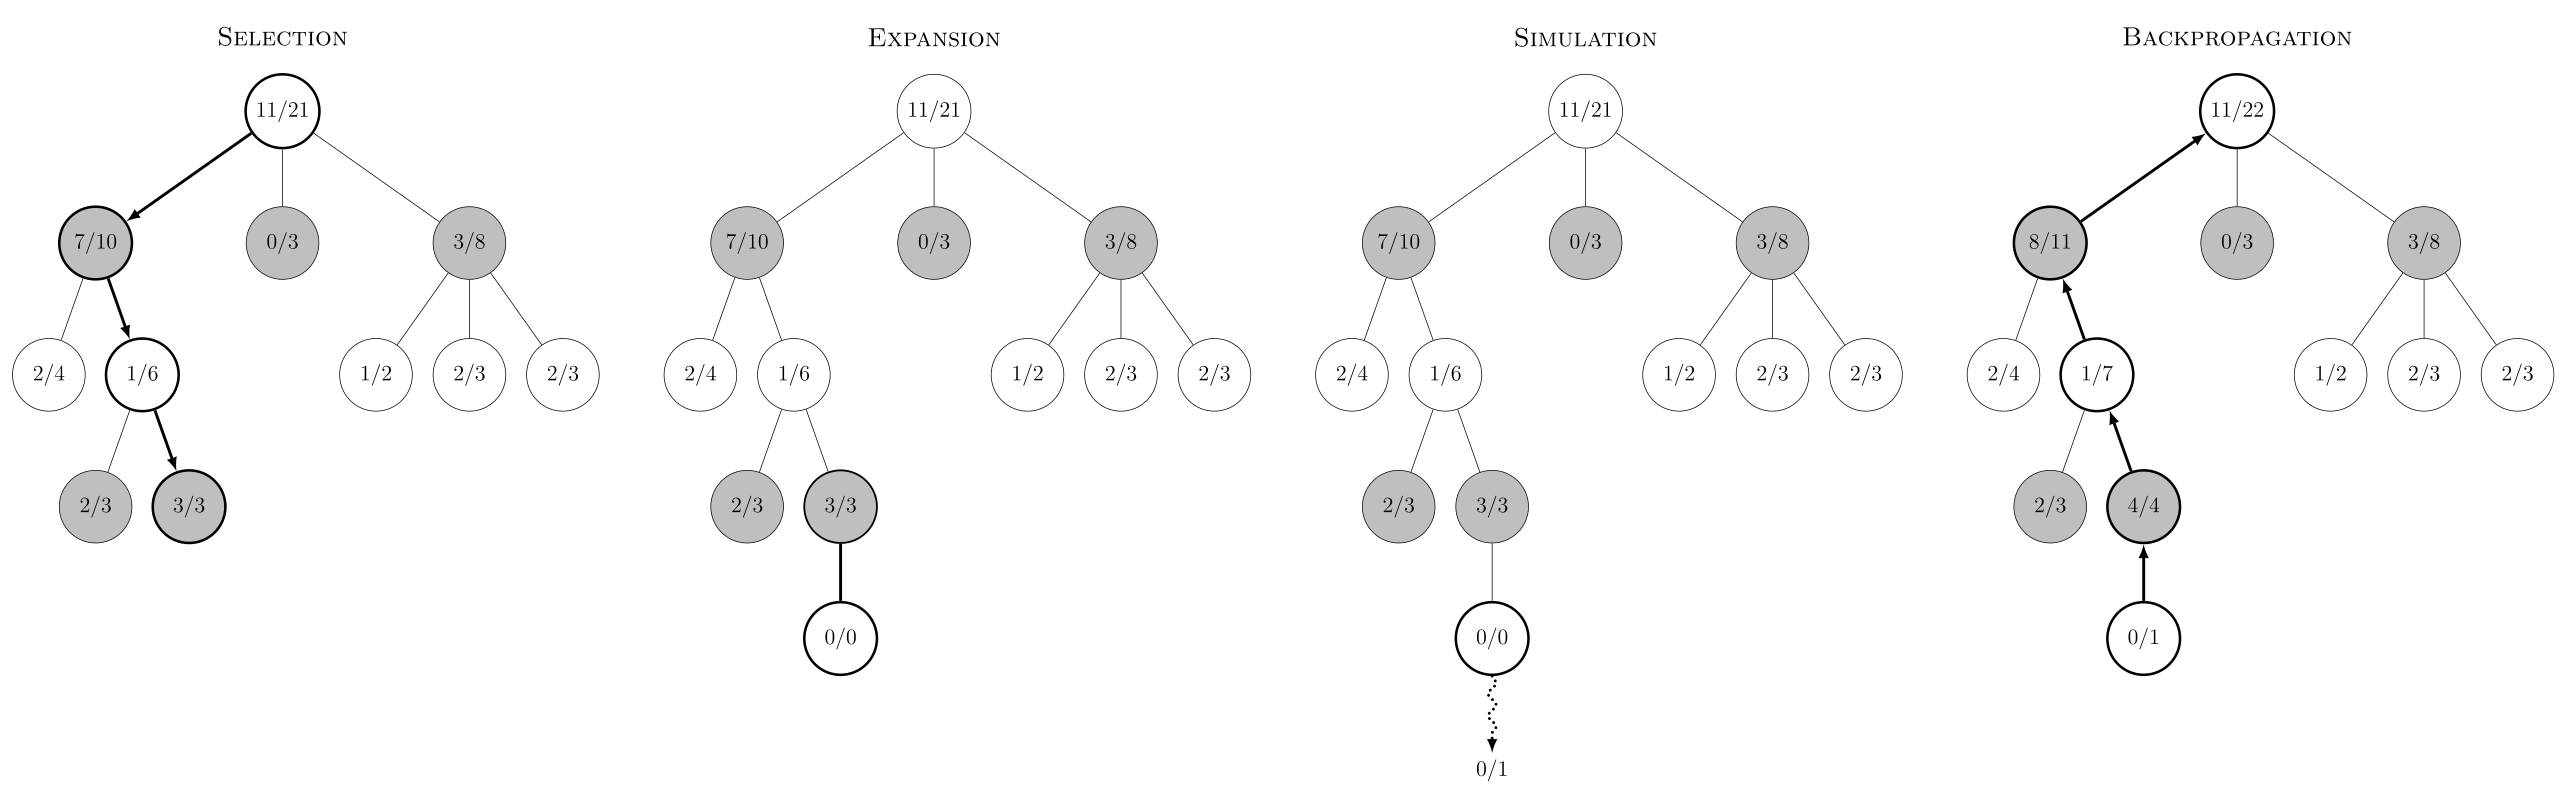
\includegraphics[width=0.98\textwidth]{img/MCTS-steps.png}
    \caption{The 4 steps of the MCTS algorithm \cite{MonteCarloTree2022}}
\end{figure}

For chess, this algorithm is very inefficient, because of its necessity to simulate 
an entire game in the third step of every simulation. 

\subsection{Go}

Go is a Chinese two-player strategy board game that uses white and black stones as playing pieces \cite{GoGame2022}.
It is played on a rectangular grid of (usually) 19 by 19 lines. The rules are relatively simple, but due to 
its extremely complex possibilities, Go has been a very popular playground for AI research similarly to chess.

\subsubsection{AlphaGo}



%%%%% Technical research %%%%%
\newpage
\section{Technical research}

%%%%% Reflection %%%%%
\newpage
\section{Reflection}

%%%%% Advice %%%%%
\newpage
\section{Advice}

%%%%% Conclusion %%%%%
\newpage
\section{Conclusion}

%%%%% Bibliography %%%%%
\newpage
\section{Bibliography}
\renewcommand{\bibname}{}
\printbibliography[heading=none]

%%%%% Appendix %%%%%
\newpage
\section{Appendix}





\end{document}